\begin{displayquote}
	\textsf{UCGLE is complex with a number of parameters which have impact on its numerical and parallel performance. The strategy of parameters' autotuing is necessary. In this chapter, we firstly introduce the autotuning scheme for each parameter, and then an adaptive UCGLE/$m$-UCGLE which is able to autune automaticly all these parameters.}
\end{displayquote}

\vspace{0.6in}

\section{Autotuning}

\begin{equation}
	cr_i=\cos\angle(r_i,r_{i-1})=\frac{||r_i||_2}{||r_{i-1}||_2}
\end{equation}

\begin{equation}
t_i=\frac{t}{m_g}
\end{equation}

\section{Heuristic for Each Parameter}
\subsection{Krylov Subspace Size}
\subsubsection{Methodology}

Autotuning of times and convergence together.

\begin{algorithm}[htbp]{}
	\caption{Autotuning Krylov subspace size of GMRES}   
	\label{alg:gmres-krylov-autotuning}   
	\begin{algorithmic}[1]
		
	\Function {Auto-Subspace}{$input$: $m_{min}$, $m_{max}$}
	\State $i=1$
	\State $m_i=m$
	\While{not converged}
		\If{$cr > cr_{max}$ or $i = 0$}
		\State $m_i=m_{max}$
		\ElsIf{$cr < cr_{min}$}
			\If{$m_{i-1} -d \geq m_{min}$}
				\State $m_i = m_{i-1}-d$
			\Else
				\State $m_i=m_{max}$
			\EndIf
		\EndIf
	\State GMRES($m_i$)
	\State $i=i+1$
	\State $cr \leftarrow \frac{||r_i||_2}{||r_{i-1}||_2}$
	\EndWhile
	\EndFunction
		
	\end{algorithmic}  
\end{algorithm}

\subsubsection{Experiments}
\subsection{LS Applied Times}
\subsubsection{Methodology}
\subsubsection{Experiments}
\subsection{LS Frequence}
\subsubsection{Methodology}
\subsubsection{Experiments}
\subsection{Number of BGMRES Components Allocated}
\subsubsection{Methodology}
\subsubsection{Experiments}
\subsection{Number of Eigenvalues}
\subsubsection{Methodology}
\subsubsection{Experiments}
\subsection{LS Plynomial Degree}
\subsubsection{Methodology}
\subsubsection{Experiments}

\section{Adaptive UCGLE/$m$-UCGLE}

\begin{figure*}[t]
	\centering
	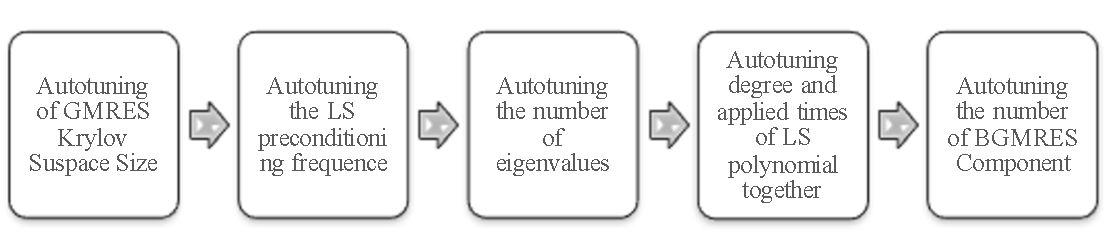
\includegraphics[width=6.3in]{fig/autotuning_order.pdf}
	\caption{The order of parameters to be autotuned.}
	\label{fig:autotuning-order}
\end{figure*}

\section{Conlusion}

\clearemptydoublepage